\id{МРНТИ 52.47.27}

{\bfseries Определение конечного коэффициента извлечения нефти при}

{\bfseries обработке воды внешним постоянным поперечным магнитным полем
малой напряженности}

{\bfseries \textsuperscript{1}А.М.
\begin{figure}[H]
	\centering
	
\includegraphics[width=0.8\textwidth]{media/gorn4/image1}
	\caption*{}
\end{figure}

\textsuperscript{2}Э.Ф.
\begin{figure}[H]
	\centering
	
\includegraphics[width=0.8\textwidth]{media/gorn4/image1}
	\caption*{}
\end{figure}

\textsuperscript{1}Т.Г.
\begin{figure}[H]
	\centering
	
\includegraphics[width=0.8\textwidth]{media/gorn4/image1}
	\caption*{}
\end{figure}

\textsuperscript{3}К.С.
\begin{figure}[H]
	\centering
	
\includegraphics[width=0.8\textwidth]{media/gorn4/image1}
	\caption*{}
\end{figure}


{\bfseries \textsuperscript{3}М.К.
\begin{figure}[H]
	\centering
	
\includegraphics[width=0.8\textwidth]{media/gorn4/image1}
	\caption*{}
\end{figure}


\emph{\textsuperscript{1}НИИ «Геотехнологические проблемы нефти, газа и
химия» г.Баку, Азербайджан,}

\emph{\textsuperscript{2}Азербайджанский Государственный университет
нефти и промышленности, Баку, Азербайджан,}

\emph{\textsuperscript{3}Южно-Казахстанский университет им. М.Ауэзова,
Шымкент, Казахстан}

{\bfseries \textsuperscript{\envelope }}Корреспондент-автор:
\href{mailto:a.k.zatybekovy@mail.ru}{\nolinkurl{a.k.zatybekovy@mail.ru}}

Данная статья посвящена изучению процесса вытеснения нефти водой,
обработанной внешним постоянным поперечным магнитным полем малой
напряженности. На нефтяных промыслах создание таких высоких
напряженностей магнитного поля сопряжено с определенными трудностями,
поэтому было решено изучить влияние магнитного поля малой напряженности
на конечный коэффициент извлечения нефти.

Для определения разности потенциалов в пористой среде предусматривалась
вольфрамовая сетка, с одной стороны, плотно примыкающая к пористой
среде, а с другой -- к проницаемой для жидкостей, изолирующей
фторопластовой прокладкой. Было обращено внимание на то, что при
изменении напряженности магнитного поля происходило изменение разности
потенциала на входе и выходе из пористой среды, которая измерялась
потенциометром. При этом максимальное значение расхода соответствовало
минимуму разности потенциала. Для получения высокой нефтеотдачи пластов
необходимо правильно выбрать напряженность магнитного поля обработки
вытесняющей воды. Экспериментально получено, что при обработке воды,
внешним постоянным поперечным магнитном полем высокой напряженностью
(H=51740 A/м и H=64476 A/м), наблюдается увеличение конечного
коэффициента извлечения нефти из пористой среды на 37\% и на 10\%
соответственно.

{\bfseries Ключевые слова:} нефть, пористая среда, коэффициент извлечения
нефти, магнитное поле, исследования, вытеснение нефти, моделирование
процесса

{\bfseries СУДЫ ТӨМЕН КЕРНЕУЛІ СЫРТҚЫ ТҰРАҚТЫ КӨЛДЕНЕҢ МАГНИТ ӨРІСІМЕН
ӨҢДЕУ КЕЗІНДЕ СОҢҒЫ МҰНАЙ АЛУ КОЭФФИЦИЕНТІН АНЫҚТАУ}

{\bfseries \textsuperscript{1}А.М. Мамед-заде, \textsuperscript{2}Э.Ф.
Ализаде, \textsuperscript{1}Т.Г. Меликов, \textsuperscript{3}К.С.
Затыбеков,}

{\bfseries \textsuperscript{3}М.К. Жантасов}

\emph{\textsuperscript{1} «Мұнай, газ және химияның геотехнологиялық
мәселелері» ҒЗИ, Баку, Әзірбайжан}

\emph{\textsuperscript{2}Әзірбайжан мемлекеттік мұнай және өнеркәсіп
университеті, Баку, Әзірбайжан}

\emph{\textsuperscript{3}М.Әуезов атындағы Оңтүстік Қазақстан
университеті, Шымкент, Қазақстан}

\emph{e-mail:
\href{mailto:a.k.zatybekovy@mail.ru}{\nolinkurl{a.k.zatybekovy@mail.ru}}}

Бұл мақала төмен кернеулі сыртқы тұрақты көлденең магнит өрісімен
өңделген мұнайды сумен ығыстыру процесін зерттеуге арналған. Мұнай
кәсіпшілігінде магнит өрісінің осындай жоғары кернеулерін құру белгілі
бір қиындықтарды тудырады, сондықтан төмен кернеулі магнит өрісінің
мұнайды алудың соңғы коэффициентіне әсерін зерттеу туралы шешім
қабылданды. Кеуекті ортадағы потенциалдар айырмашылығын анықтау үшін
вольфрам торы қарастырылды, бір жағынан кеуекті ортаға, екінші жағынан
фторопластикалық тығыздағышпен оқшауланған сұйықтық өткізгіштікке жақын.
Магнит өрісінің кернеулігі өзгерген кезде потенциометрмен өлшенетін
кеуекті ортаның кірісі мен шығуындағы потенциал айырмашылығының өзгеруі
байқалды. Бұл жағдайда ағынның максималды мәні потенциал айырмашылығының
минимумына сәйкес келді. Жоғары кернеулі сыртқы тұрақты көлденең магнит
өрісін (H=51740 A/м және H=64476 A/м) өңдеу кезінде кеуекті ортадан
мұнай алудың соңғы коэффициентінің сәйкесінше 37\% және 10\%-ға артуы
байқалды.

{\bfseries Түйін сөздер}: мұнай, кеуекті орта, мұнай алу коэффициенті,
магнит өрісі, зерттеулер, мұнайдың ығысуы, процесті модельдеу

{\bfseries DETERMINATION OF THE FINAL OIL EXTRACTION COEFFICIENT WHEN
TREATING WATER WHIT AN EXTERNAL CONSTANT TRANSVERSE MAGNETIC FIELD OF
LOW STRENGTH}

{\bfseries \textsuperscript{1}A.M.Mammad-zade,
\textsuperscript{2}E.F.Alizadeh, \textsuperscript{1}T.G.Melikov,
\textsuperscript{3}K.S.Zatybekov,}

{\bfseries \textsuperscript{3}M.K.Zhantasov}

\emph{\textsuperscript{1}Research Institute "Geotechnological Problems
of oil, gas and chemistry" Baku, Azerbaijan}

\emph{\textsuperscript{2}Azerbaijan State University of Petroleum and
Industry, Baku, Azerbaijan}

\emph{\textsuperscript{3}M.Auezov South Kazakhstan University, Shymkent,
Kazakhstan}

\emph{e-mail:
\href{mailto:a.k.zatybekovy@mail.ru}{\nolinkurl{a.k.zatybekovy@mail.ru}}}

This article is devoted to the study of the process of oil displacement
by water treated with an external permanent transverse magnetic field of
low intensity. In oil fields, the creation of such high magnetic field
strengths is fraught with certain difficulties, so it was decided to
study the effect of a low-intensity magnetic field on the final oil
recovery coefficient. To determine the potential difference in a porous
medium, a tungsten mesh was provided, on the one hand, tightly adjacent
to the porous medium, and on the other, to a liquid--permeable,
insulating fluoroplastic gasket. Attention was drawn to the fact that
when the magnetic field strength changed, there was a change in the
potential difference at the entrance and exit from the porous medium,
which was measured by a potentiometer. At the same time, the maximum
flow rate corresponded to the minimum potential difference. To obtain
high reservoir recoil oil, it is necessary to choose the right magnetic
field strength for the treatment of displacing water. It has been
experimentally obtained that when water is treated with an external
constant transverse magnetic field of high intensity (H=51740 A/m and
H=64476 A/m), an increase in the final coefficient of oil extraction
from a porous medium is observed by 37\% and 10\%, respectively.

{\bfseries Keywords}: oil, porous medium, oil recovery coefficient,
magnetic field, research, oil displacement, process modeling

{\bfseries Введение.} Современное состояние разработки нефтяных
месторождений характеризуется необходимостью извлечения
трудноизвлекаемых запасов, особенно на поздних стадиях эксплуатации, где
традиционные методы заводнения становятся недостаточно эффективными.
Повышение коэффициента извлечения нефти (КИН) остается одной из
приоритетных задач нефтедобывающей отрасли. Одним из альтернативных и
энергосберегающих подходов к увеличению нефтеотдачи является
использование физических методов воздействия на вытесняющие агенты,
включая магнитную обработку воды.

Создание высоких напряженностей магнитного поля на промыслах сопряжено с
техническими и энергетическими трудностями. Поэтому интерес представляет
изучение влияния магнитного поля малой напряженности на процессы
вытеснения нефти. Несмотря на наличие работ, посвященных магнитной
обработке жидкости, влияние слабых полей на фильтрационные
характеристики и поведение жидкостей в пористой среде недостаточно
изучено и требует дополнительных исследований.

{\bfseries Актуальность} данного исследования обусловлена: необходимостью
повышения нефтеотдачи в условиях зрелых и малодебитных коллекторов;
отсутствием однозначных данных по влиянию слабых магнитных полей на
коэффициент извлечения нефти; потенциальной возможностью промышленного
применения магнитной обработки воды как недорогого и экологически
безопасного метода интенсификации добычи.

{\bfseries Цель работы} - определить влияние малых напряженностей
магнитного поля на коэффициент извлечения нефти при вытеснении её водой,
предварительно обработанной магнитным полем.

{\bfseries Задачи исследования:}

\begin{enumerate}
\def\labelenumi{\arabic{enumi}.}
\item
  Провести физическое моделирование вытеснения нефти в лабораторных
  условиях.
\item
  Изучить влияние различных значений напряженности магнитного поля (H =
  7980; 11970; 15960 A/м) на конечный коэффициент извлечения нефти.
\item
  Проанализировать механизм взаимодействия магнитного поля с системой
  "нефть--пористая среда--вода", включая электрокинетические явления.
\item
  Сопоставить полученные результаты с данными из литературных источников
  и выявить наиболее эффективный диапазон значений магнитного
  воздействия.
\item
  Оценить возможность промышленного применения метода для различных
  типов коллекторов.
\end{enumerate}

{\bfseries Научная новизна.} Впервые экспериментально исследовано влияние
слабого магнитного поля на коэффициент извлечения нефти в диапазоне H =
7980--15960 А/м.

Определены интервалы напряженности, оказывающие как положительное, так и
отрицательное влияние на процесс вытеснения.

Раскрыт механизм изменения потенциала и поведения двойного
электрического слоя под действием магнитного поля.

{\bfseries Литературный обзор.} Повышение коэффициента извлечения нефти ---
одна из важнейших задач нефтяной отрасли. Среди множества методов всё
большее внимание уделяется физическим воздействиям, включая
акустическое, тепловое, виброволновое и магнитное. Магнитная обработка
воды привлекает внимание исследователей как энергетически эффективный и
технологически простой способ увеличения нефтеотдачи.

Согласно работе {[}1{]}, магнитное воздействие может изменять
физико-химические свойства воды: поверхностное натяжение, вязкость,
способность к смачиванию. Это подтверждается экспериментами {[}2{]}, где
магнитно-обработанная вода способствовала повышению нефтеотдачи в
условиях низкопроницаемых коллекторов. В работе {[}3{]}
продемонстрировали значительное улучшение смачиваемости карбонатных
пород при использовании воды, обработанной магнитным полем.

Авторы {[}4,5{]} исследовали влияние магнитного воздействия на межфазное
натяжение и показали, что оптимальные значения напряженности магнитного
поля позволяют достичь максимального эффекта за счет изменения свойств
двойного электрического слоя.

В ряде случаев использование магнитной обработки воды дало отрицательный
эффект, что обусловлено ошибками моделирования или неучетом особенностей
взаимодействия физического поля с жидкой средой. Поэтому необходим
критический подход и точная калибровка параметров.Автором {[}6,7{]}
экспериментально получено, что при обработке воды, внешним постоянным
поперечным магнитным полем высокой напряженностью H=51740 A/м и H=64476
A/м наблюдается увеличение конечного коэффициента извлечения нефти из
пористой среды на 37\% и на 10\% соответственно.

В работе {[}6,8{]} показана зависимость расхода воды на выходе из
пористой среды от напряженности внешнего постоянного магнитного поля.
При этом, график Q -- H состоит из трёх областей: 1- ниже оси OX (H),
область малых напряженностей магнитного поля; 2- по оси OX, область
отсутствия влияния магнитного поля; 3- выше оси OX (H), область высоких
напряженностей магнитного поля, которая изучена в {[}8-11{]}.

Ряд авторов {[}11,12{]} отмечают сложность повторяемости эффекта и
наличие полиэкстремальных зависимостей между напряженностью поля и
эффектом нефтеотдачи. Это подчеркивает важность экспериментальной
проверки конкретных значений напряженности магнитного поля в разных
горно-геологических условиях.

Возникла мысль: как зависит конечный коэффициент извлечения нефти из
пористой среде при малых значениях напряженности магнитного поля, что
рассмотрено далее в предложенной статье.

{\bfseries Материалы и методы.} Исследования поставленного выше вопроса
осуществлялось физическим моделированием процесса в лаборатории
вытеснением нефти водой из пористой среды. При этом соблюдались
параметры моделирования процесса с учетом критериев подобия, приведенных
в {[}13-14{]}.

\begin{figure}[H]
	\centering
	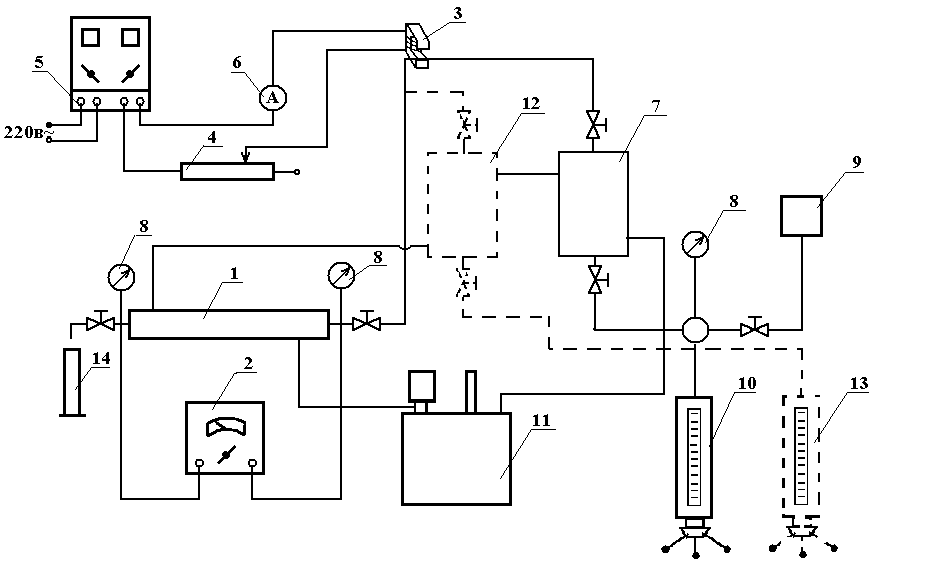
\includegraphics[width=0.8\textwidth]{media/gorn4/image2}
	\caption*{}
\end{figure}


{\bfseries Рис. 1 - Схема экспериментальной установки}

Эксперименты проводились на лабораторной установке, схема которой
рприведена на рис. 1, состоящей из: колонки высокого давления (1),
потенциометра с высоким входным сопротивлением URV-2M (2);
электромагнита со специальным наконечником (3); реостата (4);
выпрямителя типа УСА-4А (5); вольтамперметра (6); бомбы высокого
давления типа PVT (7 и 12); образцовых манометров (8); бачка для
жидкости (9), с помощью которой заполняется очередная порция пресса;
измерительного пресса (10 и 13); термостата (11). В бомбах PVT (7 и 12)
и колонке высокого давления (1) с помощью термостата (11) поддерживается
постоянная температура которая была 313 К.

Колонка высокого давления представляет собой полный цилиндр с внутренним
диаметром 31 мм и длиной рабочей части 1100 мм и уплотняется резиновыми
кольцами с сальниковым уплотнением. Размеры получены с учетом критериев
подобия, приведенных в работе {[}15-16{]}.

Для определения разности потенциалов в пористой среде предусматривается
вольфрамовая сетка, с одной стороны, плотно примыкающая к пористой
среде, а с другой -- к проницаемой для жидкостей, изолирующей
фторопластовой прокладкой. Таким образом, осуществляется изоляция
пористой среды с торцевых концов металлической колонки высокого давления
(1). Изоляция потенциала протекания пористой среды (U) от корпуса
колонки (1) осуществлялась эпоксидным клеем, наносимым на внутреннюю
поверхность колонки, склеивающий слой песка с металлической
поверхностью. Этим также предотвращается просачивание жидкости между
пористой средой и корпусом колонки. В противном случае, пористая среда
не насыщается (не заполняется) исследуемой жидкостью, остаётся сухой; в
этом случае эксперимент нельзя проводить.

Вольфрамовая сетка с помощью изолированных проводов соединяется с
потенциометром (2), которым осуществляется измерение разности
потенциалов между торцами пористой среды. Эксперименты проводились
следующим образом:

1. Колонку высокого давления (1) заполняли пористой средой вертикально
вибрационной трамбовкой с дополнением каждый раз новой порции пористой
среды, после чего создавали горное давление ввинчиванием верхнего фланца
колонки. Колонку заполняли до тех пор, пока вибрация и создаваемое
горное давление не переставали влиять на степень уплотнения пористой
среды. Таким образом, получали образец с постоянной проницаемостью, не
зависящей от давления.

2. После уплотнения пористой среды в колонне высокого давления
определяли воздухопроницаемостью породы. Воздухопроницаемость пористой
среды определяли использованием известного метода {[}9,18{]}. Объем пор
определялся как весовым способом, так и вычислялся по уравнению
состояния газа {[}19-21{]}.

3. Пористую среду с помощью бомбы PVT (7) насыщали исследуемой нефтью.
Для этого пористую среду предварительно вакуумировали. Через пористую
среду прокачали десять поровых объёмов исследуемой жидкости. При
прокачке исследуемой жидкости в системе периодически повышали давление и
резко выпускали жидкость для лучшей очистки пористой среды от газа: за
счет частичного его растворения при повышении давления в колонке, а
также за счет проскальзывания газа при больших перепадах давления в
колонке за счет снижения давления на выходе из колонки.

4. Бомбу PVT (12) соединяют водой, которой будет осуществляться
вытеснение нефти из модели пласта.

5. Бомбу PVT (12) соединяют с моделью пласта (1) и производят вытеснение
нефти водой.

6. На выходе из модели пласта (1) с помощью мензурки (14) (периодически
с помощью секундомера) замеряют количество вытесняемой нефти и
рассчитывают коэффициент измерения нефти --\(\eta\)\textsubscript{i}.

7. Вытеснение нефти из модели пласта (1) осуществляют до тех пор, пока
на выходе из колонки будет выходить только вода.

8. После окончания эксперимента колонку модели пласта (1) освобождают от
отработанной пористой среды и производят подготовку к следующему
эксперименту.

9. После проведения подготовительной работы пункты 1-4, производят
эксперимент 2, аналогично предыдущему.

10. Бомбу PVT(7) заполняют исследуемой нефтью.

11. Из бомбы PVT (7) нефть переводят в модель пласта (1), по выше
приведенной методике (пункт 4).

12. Бомбу НTР (12) заполняют водой, которой будет осуществляется
вытеснение нефти из модели пласта.

13. Бомбу PVT (12) соединяют с моделью пласта (1), при этом, медная
трубочка, соединяющая бомбу PVT (12) с колонкой высокого давления (1),
вставляется в зазор сердечника электромагнита (3) аналогично соединению
бомбы Бомбу PVT (7) как показано на рис. 1.

14. Выпрямитель типа USA -- 4A (5) включается в электрическую сеть
переменного тока.

15. На выходе выпрямитель (5) получаем постоянный ток, который подается
в электрическую цепь электромагнита (3).

16. С помощью реостата (4) и амперметра (6) в зазоре электромагнита (3)
устанавливается определенная напряженность магнитного поля
H\textsubscript{i}.

17. При протекании воды в медной трубочке, происходит обработка её
перпендикулярным поперечным магнитным полем.

18. Производят вытеснение нефти намагниченной водой.

19. На выходе из модели пласта (1) с помощью мензурки (14) (периодически
с помощью секундомера) замеряют количество вытесняемой нефти
Q\textsubscript{i}и рассчитывают коэффициент конечного извлечения нефти
- \(\eta\)\textsubscript{i}.

20. Результаты пункта 7 и 20 заносятся в таблицы 1,2,3,4.

{\bfseries Результаты и обсуждение.} В лабораторных условиях каждый
эксперимент по вытеснению нефти из пористой среды, в лучшем случае
осуществляется в течение одного месяца и более. Для получения ответа на
поставленный в статье вопрос в кратчайшее время, чтобы не дублировать
опыты, приведенные в {[}1,3,5{]}, было решено воспользоваться их
результатами. Экспериментальная установка и методика проведения
экспериментов была аналогичной {[}1,2{]}. В данной работе приведена
зависимость расхода от напряженности магнитного поля, снятая длямагнит
обработанной воды в карбонатной пористой среде при постоянном перепаде
давлений 0,4 МПа. Приведенная на рис.2 зависимость наглядно показывает,
что существуют интервалы напряженностей, когда следует ожидать
отрицательного воздействия от магнитной обработки. В рассматриваемом
случае что H = 9950 -- 19900 А/м. Было обращено внимание на то, что при
изменении напряженности магнитного поля происходило изменение разности
потенциала на входе и выходе из пористой среды, которая измерялась
потенциометром (2). При этом максимальное значение расхода
соответствовало минимуму разности потенциала. В работе {[}5{]} академика
Фрумкина А.Н. указывается, что потенциал протекания зависит от состояния
поверхности и его заряда, причем имеется максимум на зависимости расхода
от заряда.

\begin{figure}[H]
	\centering
	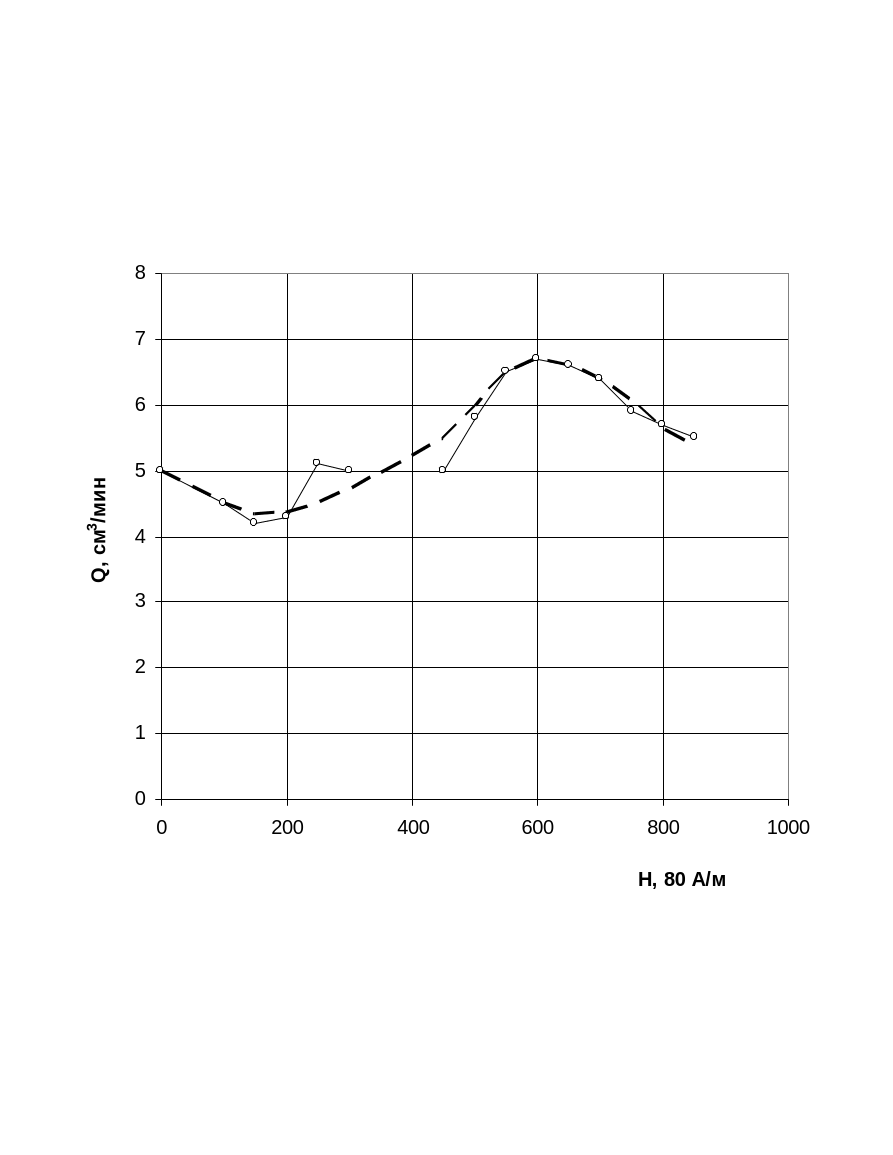
\includegraphics[width=0.8\textwidth]{media/gorn4/image3}
	\caption*{}
\end{figure}


{\bfseries Рис. 2 -- Зависимость расхода Q от напряженности магнитного поля
Н {[}1,2{]}}

Из рисунка 2 следует, что в нашем случае, область малых напряженностей
магнитного поля находится в интервале 0÷19950 А/м. Исходя из этого, было
решенопроводить вытеснение нефти из модели пласта водой и водой,
обработанной магнитным полем:H=7980; 11970; 15960 A/м.

В качестве модели пласта была взята смесь: кварцевого песка (50\%) плюс
(50\%) карбоната, аналогичная пористой среде в работе {[}6, 12{]}.
Результаты экспериментов приведены в таблице 1 -- 4. Результаты
вытеснения нефти водой приведены в таблице 1.

{\bfseries Таблица 1 - Результаты вытеснения нефти водой}

% \begin{longtable}[]{@{}
%   >{\raggedright\arraybackslash}p{(\columnwidth - 26\tabcolsep) * \real{0.0814}}
%   >{\raggedright\arraybackslash}p{(\columnwidth - 26\tabcolsep) * \real{0.0666}}
%   >{\raggedright\arraybackslash}p{(\columnwidth - 26\tabcolsep) * \real{0.0695}}
%   >{\raggedright\arraybackslash}p{(\columnwidth - 26\tabcolsep) * \real{0.0716}}
%   >{\raggedright\arraybackslash}p{(\columnwidth - 26\tabcolsep) * \real{0.0685}}
%   >{\raggedright\arraybackslash}p{(\columnwidth - 26\tabcolsep) * \real{0.0716}}
%   >{\raggedright\arraybackslash}p{(\columnwidth - 26\tabcolsep) * \real{0.0716}}
%   >{\raggedright\arraybackslash}p{(\columnwidth - 26\tabcolsep) * \real{0.0718}}
%   >{\raggedright\arraybackslash}p{(\columnwidth - 26\tabcolsep) * \real{0.0715}}
%   >{\raggedright\arraybackslash}p{(\columnwidth - 26\tabcolsep) * \real{0.0716}}
%   >{\raggedright\arraybackslash}p{(\columnwidth - 26\tabcolsep) * \real{0.0706}}
%   >{\raggedright\arraybackslash}p{(\columnwidth - 26\tabcolsep) * \real{0.0717}}
%   >{\raggedright\arraybackslash}p{(\columnwidth - 26\tabcolsep) * \real{0.0716}}
%   >{\raggedright\arraybackslash}p{(\columnwidth - 26\tabcolsep) * \real{0.0704}}@{}}
% \toprule\noalign{}
% \begin{minipage}[b]{\linewidth}\raggedright
% t,мин.
% \end{minipage} & \begin{minipage}[b]{\linewidth}\raggedright
% 0
% \end{minipage} & \begin{minipage}[b]{\linewidth}\raggedright
% 32
% \end{minipage} & \begin{minipage}[b]{\linewidth}\raggedright
% 56
% \end{minipage} & \begin{minipage}[b]{\linewidth}\raggedright
% 96
% \end{minipage} & \begin{minipage}[b]{\linewidth}\raggedright
% 120
% \end{minipage} & \begin{minipage}[b]{\linewidth}\raggedright
% 136
% \end{minipage} & \begin{minipage}[b]{\linewidth}\raggedright
% 176
% \end{minipage} & \begin{minipage}[b]{\linewidth}\raggedright
% 256
% \end{minipage} & \begin{minipage}[b]{\linewidth}\raggedright
% 312
% \end{minipage} & \begin{minipage}[b]{\linewidth}\raggedright
% 440
% \end{minipage} & \begin{minipage}[b]{\linewidth}\raggedright
% 540
% \end{minipage} & \begin{minipage}[b]{\linewidth}\raggedright
% 768
% \end{minipage} & \begin{minipage}[b]{\linewidth}\raggedright
% 768
% \end{minipage} \\
% \midrule\noalign{}
% \endhead
% \bottomrule\noalign{}
% \endlastfoot
% \(\eta\) & 0 & 6.3 & 11.8 & 20 & 24.7 & 26.3 & 31.4 & 33.3 & 35.3 & 39 &
% 41.2 & 41.2 & 49 \\
% \end{longtable}

{\bfseries Таблица 2- Результаты вытеснения нефти водой, обработанной
магнитным полем напряженностью H=7980 A/м}

% \begin{longtable}[]{@{}
%   >{\raggedright\arraybackslash}p{(\columnwidth - 24\tabcolsep) * \real{0.1024}}
%   >{\raggedright\arraybackslash}p{(\columnwidth - 24\tabcolsep) * \real{0.0643}}
%   >{\raggedright\arraybackslash}p{(\columnwidth - 24\tabcolsep) * \real{0.0727}}
%   >{\raggedright\arraybackslash}p{(\columnwidth - 24\tabcolsep) * \real{0.0796}}
%   >{\raggedright\arraybackslash}p{(\columnwidth - 24\tabcolsep) * \real{0.0698}}
%   >{\raggedright\arraybackslash}p{(\columnwidth - 24\tabcolsep) * \real{0.0753}}
%   >{\raggedright\arraybackslash}p{(\columnwidth - 24\tabcolsep) * \real{0.0795}}
%   >{\raggedright\arraybackslash}p{(\columnwidth - 24\tabcolsep) * \real{0.0753}}
%   >{\raggedright\arraybackslash}p{(\columnwidth - 24\tabcolsep) * \real{0.0797}}
%   >{\raggedright\arraybackslash}p{(\columnwidth - 24\tabcolsep) * \real{0.0753}}
%   >{\raggedright\arraybackslash}p{(\columnwidth - 24\tabcolsep) * \real{0.0752}}
%   >{\raggedright\arraybackslash}p{(\columnwidth - 24\tabcolsep) * \real{0.0756}}
%   >{\raggedright\arraybackslash}p{(\columnwidth - 24\tabcolsep) * \real{0.0751}}@{}}
% \toprule\noalign{}
% \begin{minipage}[b]{\linewidth}\raggedright
% t,мин.
% \end{minipage} & \begin{minipage}[b]{\linewidth}\raggedright
% 0
% \end{minipage} & \begin{minipage}[b]{\linewidth}\raggedright
% 40
% \end{minipage} & \begin{minipage}[b]{\linewidth}\raggedright
% 60
% \end{minipage} & \begin{minipage}[b]{\linewidth}\raggedright
% 93
% \end{minipage} & \begin{minipage}[b]{\linewidth}\raggedright
% 120
% \end{minipage} & \begin{minipage}[b]{\linewidth}\raggedright
% 130
% \end{minipage} & \begin{minipage}[b]{\linewidth}\raggedright
% 170
% \end{minipage} & \begin{minipage}[b]{\linewidth}\raggedright
% 250
% \end{minipage} & \begin{minipage}[b]{\linewidth}\raggedright
% 300
% \end{minipage} & \begin{minipage}[b]{\linewidth}\raggedright
% 470
% \end{minipage} & \begin{minipage}[b]{\linewidth}\raggedright
% 520
% \end{minipage} & \begin{minipage}[b]{\linewidth}\raggedright
% 780
% \end{minipage} \\
% \midrule\noalign{}
% \endhead
% \bottomrule\noalign{}
% \endlastfoot
% \(\eta\) & 0 & 5.5 & 10.5 & 18 & 22 & 23.5 & 28 & 29.5 & 31 & 35 & 37 &
% 44 \\
% \end{longtable}

{\bfseries Таблица 3- Результаты вытеснения нефти водой, обработанной
магнитным полем напряженностью H=11970 A/м}

% \begin{longtable}[]{@{}
%   >{\raggedright\arraybackslash}p{(\columnwidth - 24\tabcolsep) * \real{0.1026}}
%   >{\raggedright\arraybackslash}p{(\columnwidth - 24\tabcolsep) * \real{0.0646}}
%   >{\raggedright\arraybackslash}p{(\columnwidth - 24\tabcolsep) * \real{0.0723}}
%   >{\raggedright\arraybackslash}p{(\columnwidth - 24\tabcolsep) * \real{0.0783}}
%   >{\raggedright\arraybackslash}p{(\columnwidth - 24\tabcolsep) * \real{0.0698}}
%   >{\raggedright\arraybackslash}p{(\columnwidth - 24\tabcolsep) * \real{0.0760}}
%   >{\raggedright\arraybackslash}p{(\columnwidth - 24\tabcolsep) * \real{0.0792}}
%   >{\raggedright\arraybackslash}p{(\columnwidth - 24\tabcolsep) * \real{0.0757}}
%   >{\raggedright\arraybackslash}p{(\columnwidth - 24\tabcolsep) * \real{0.0796}}
%   >{\raggedright\arraybackslash}p{(\columnwidth - 24\tabcolsep) * \real{0.0756}}
%   >{\raggedright\arraybackslash}p{(\columnwidth - 24\tabcolsep) * \real{0.0751}}
%   >{\raggedright\arraybackslash}p{(\columnwidth - 24\tabcolsep) * \real{0.0753}}
%   >{\raggedright\arraybackslash}p{(\columnwidth - 24\tabcolsep) * \real{0.0758}}@{}}
% \toprule\noalign{}
% \begin{minipage}[b]{\linewidth}\raggedright
% t,мин.
% \end{minipage} & \begin{minipage}[b]{\linewidth}\raggedright
% 0
% \end{minipage} & \begin{minipage}[b]{\linewidth}\raggedright
% 31
% \end{minipage} & \begin{minipage}[b]{\linewidth}\raggedright
% 55
% \end{minipage} & \begin{minipage}[b]{\linewidth}\raggedright
% 95
% \end{minipage} & \begin{minipage}[b]{\linewidth}\raggedright
% 120
% \end{minipage} & \begin{minipage}[b]{\linewidth}\raggedright
% 130
% \end{minipage} & \begin{minipage}[b]{\linewidth}\raggedright
% 174
% \end{minipage} & \begin{minipage}[b]{\linewidth}\raggedright
% 230
% \end{minipage} & \begin{minipage}[b]{\linewidth}\raggedright
% 280
% \end{minipage} & \begin{minipage}[b]{\linewidth}\raggedright
% 400
% \end{minipage} & \begin{minipage}[b]{\linewidth}\raggedright
% 490
% \end{minipage} & \begin{minipage}[b]{\linewidth}\raggedright
% 700
% \end{minipage} \\
% \midrule\noalign{}
% \endhead
% \bottomrule\noalign{}
% \endlastfoot
% \(\eta\) & 0 & 5.3 & 10 & 16 & 20.5 & 22 & 26.5 & 28.5 & 30 & 34 & 37 &
% 41.5 \\
% \end{longtable}

{\bfseries Таблица 4- Результаты вытеснения нефти водой, обработанной
магнитным полем напряженностью H=15960 A/м}

% \begin{longtable}[]{@{}
%   >{\raggedright\arraybackslash}p{(\columnwidth - 24\tabcolsep) * \real{0.1025}}
%   >{\raggedright\arraybackslash}p{(\columnwidth - 24\tabcolsep) * \real{0.0645}}
%   >{\raggedright\arraybackslash}p{(\columnwidth - 24\tabcolsep) * \real{0.0726}}
%   >{\raggedright\arraybackslash}p{(\columnwidth - 24\tabcolsep) * \real{0.0795}}
%   >{\raggedright\arraybackslash}p{(\columnwidth - 24\tabcolsep) * \real{0.0701}}
%   >{\raggedright\arraybackslash}p{(\columnwidth - 24\tabcolsep) * \real{0.0752}}
%   >{\raggedright\arraybackslash}p{(\columnwidth - 24\tabcolsep) * \real{0.0796}}
%   >{\raggedright\arraybackslash}p{(\columnwidth - 24\tabcolsep) * \real{0.0754}}
%   >{\raggedright\arraybackslash}p{(\columnwidth - 24\tabcolsep) * \real{0.0792}}
%   >{\raggedright\arraybackslash}p{(\columnwidth - 24\tabcolsep) * \real{0.0753}}
%   >{\raggedright\arraybackslash}p{(\columnwidth - 24\tabcolsep) * \real{0.0752}}
%   >{\raggedright\arraybackslash}p{(\columnwidth - 24\tabcolsep) * \real{0.0756}}
%   >{\raggedright\arraybackslash}p{(\columnwidth - 24\tabcolsep) * \real{0.0751}}@{}}
% \toprule\noalign{}
% \begin{minipage}[b]{\linewidth}\raggedright
% t,мин.
% \end{minipage} & \begin{minipage}[b]{\linewidth}\raggedright
% 0
% \end{minipage} & \begin{minipage}[b]{\linewidth}\raggedright
% 30
% \end{minipage} & \begin{minipage}[b]{\linewidth}\raggedright
% 54
% \end{minipage} & \begin{minipage}[b]{\linewidth}\raggedright
% 94
% \end{minipage} & \begin{minipage}[b]{\linewidth}\raggedright
% 120
% \end{minipage} & \begin{minipage}[b]{\linewidth}\raggedright
% 133
% \end{minipage} & \begin{minipage}[b]{\linewidth}\raggedright
% 175
% \end{minipage} & \begin{minipage}[b]{\linewidth}\raggedright
% 250
% \end{minipage} & \begin{minipage}[b]{\linewidth}\raggedright
% 300
% \end{minipage} & \begin{minipage}[b]{\linewidth}\raggedright
% 420
% \end{minipage} & \begin{minipage}[b]{\linewidth}\raggedright
% 500
% \end{minipage} & \begin{minipage}[b]{\linewidth}\raggedright
% 720
% \end{minipage} \\
% \midrule\noalign{}
% \endhead
% \bottomrule\noalign{}
% \endlastfoot
% \(\eta\) & 0 & 5.4 & 10.2 & 17 & 21 & 22.5 & 27 & 30 & 32 & 35 & 38 &
% 42 \\
% \end{longtable}

\emph{{\bfseries Анализ полученных данных.}} Для оценки влияния магнитного
поля на процесс вытеснения нефти из модели пласта произведем
сопоставление результатов, полученных при вытеснении водой с
результаттами, полученными при вытеснении намагниченной водой. Построим
график используя таблицы: 1-2 (рис.3); 1-3 (рис.4); 1-4 (рис.5)

\begin{figure}[H]
	\centering
	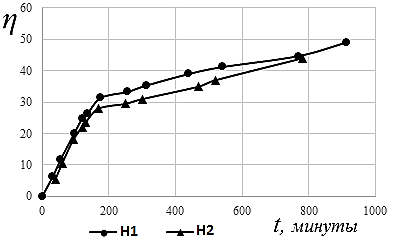
\includegraphics[width=0.8\textwidth]{media/gorn4/image4}
	\caption*{}
\end{figure}


{\bfseries Рис.3 - Сопоставление} \(\eta\) {\bfseries при вытеснении водой
(H\textsubscript{1}=0) и намагниченной водой (H\textsubscript{2}=7980
А/м)}

\begin{figure}[H]
	\centering
	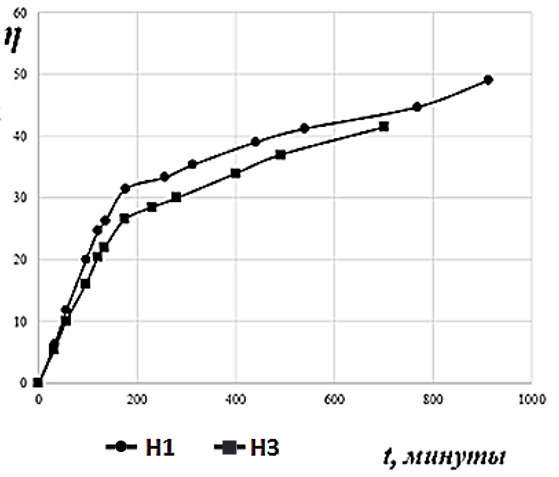
\includegraphics[width=0.8\textwidth]{media/gorn4/image5}
	\caption*{}
\end{figure}


{\bfseries Рис.4 - Сопоставление} \(\eta\) {\bfseries при вытеснении водой
(H\textsubscript{1}=0) и намагниченной водой (H\textsubscript{3}=11970
А/м)}

{\bfseries Рис.5 - Сопоставление} \(\eta\) {\bfseries при вытеснении водой
(H\textsubscript{1}=0) и намагниченной водой
\begin{figure}[H]
	\centering
	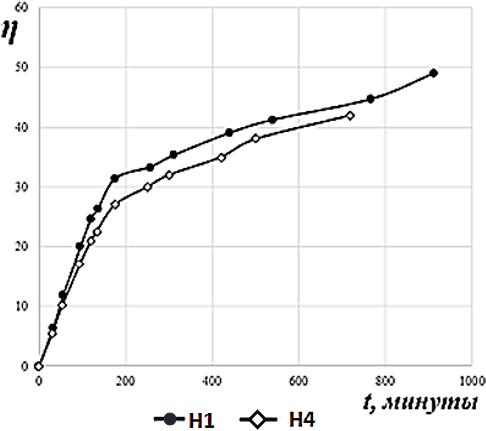
\includegraphics[width=0.8\textwidth]{media/gorn4/image6}
	\caption*{}
\end{figure}

А/м)}

Из рисунка 3 следует, что при вытеснении нефти водой, предварительно
обработанной постоянным поперечным магнитным полем напряженностью 7980
А/м, происходит уменьшение коэффициента вытеснения нефти на 5\% по
сравнению с вытеснением такой же нефти такой же водой из аналогичной
пористой среды.

Из рисунка 4 следует, что при вытеснении нефти водой, предварительно
обработанной постоянным поперечным магнитным полем напряженностью 11970
А/м, происходит уменьшение коэффициента вытеснения нефти на 7,5\% по
сравнению с вытеснением такой же нефти такой же водой из аналогичной
пористой среды.

Из рисунка 5 следует, что при вытеснении нефти водой, предварительно
обработанной постоянным поперечным магнитным полем напряженностью 15960
А/м, происходит уменьшение коэффициента вытеснения нефти на 7\% по
сравнению с вытеснением такой же нефти такой же водой из аналогичной
пористой среды.

Из курса «Физической химии» известно, что нефть на поверхности породы
образует двойной электрический слой, толщину которого можно изменять
различным видом воздействия, в том числе и магнитным полем. В нашем
случае, при малых величинах напряженности магнитного поля его не
достаточно для полной компенсации поля породы. Это приводит к снижению
коэффициента вытеснения нефти по сравнению с вытеснением водой. В том
случае, когда напряженность магнитного поля высокая (смотри стр.75
{[}1{]}), то происходит полная компенсация поля породы, тогда получаем
максимальное увеличение коэффициента извлечения нефти.

{\bfseries Выводы:} Для получения высокого коэффициента нефтеотдачи пластов
необходимо правильно выбрать напряженность магнитного поля обработки
вытесняющей воды. Для исследуемой пористой среды напряженность
магнитного поля обработки вытесняющей воды H=51740А/м.

В процессе перфорации скважины глубокое внедрение буровой жидкости в
пласт не желательно. В этом случае, буровой раствор обрабатывается
магнитным полем напряженностью H=11970А/м.

Сравнение опытных результатов рисунков 3, 4, 5 и 25 стр.75 {[}1{]} по
вытеснению нефти из глинизированной пористой среды с результатами рис.2
зависимости расхода нефти при фильтрации из аналогичной пористой среды
показал, что в интервале напряженностей H = 9950 -- 19900 А/м
наблюдается отрицательное воздействие от магнитной обработки воды.

{\bfseries Литература}

1.Bahadori, A. Fundamentals of Enhanced Oil and Gas Recovery from
Conventional and Unconventional Reservoirs. Elsevier.-2018.-522p.
\href{https://doi.org/10.1016/C2016-0-04615-6}{DOI
10.1016/C2016-0-04615-6}

2.Zhang, Y., Wang, J., Liu, Z. et al. (2016). "Experimental
Investigation on Magnetic Water Flooding for Enhanced Oil
Recovery.//Journal of Petroleum Science and Engineering.-Vol. 145.- 487
- 494. DOI
\href{https://doi.org/10.1016/j.petrol.2016.05.036}{10.1016/j.petrol.2016.05.036}

3.Nasralla, R. A., \& Nasr-El-Din, H. A. (2015). "Impact of Magnetic
Field on the Properties of Injection Water and Enhanced Oil Recovery in
Carbonate Reservoirs// SPE Journal.-Vol. 20(04).- 760 - 772. DOI
10.2118/169107-PA

4.Li, X., Liu, Y., Song, Y. et al. (2020). "Magnetic Water Flooding:
Effects on Oil Recovery and Reservoir Properties//Fuel.-Vol. 262:116580.
DOI 10.1016/j.fuel.2019.116580

5.Tang, D., Zhang, M., Zhao, Y. et al. Mechanism Study of Magnetic
Treatment on Water and Its Effects on the Interfacial Tension in Oil
Recovery//Colloids and Surfaces A: Physicochemical and Engineering
A.-spects.-2018.-Vol.538.-P. 765--773.

\href{https://doi.org/10.1016/j.colsurfa.2017.11.051}{DOI
10.1016/j.colsurfa.2017.11.051}

6.Мамед-заде А.М. Нанотехнологии в нефтедобыче. Баку: Uniprint, 2010.
264 c.

7.T.A. Mammadova, M.M. Abbasov, I.A. Safarli, Kh.Sh. Teyubov, N.E.
Asgarli, V.M.Abbasov. The influence of magnetic field on the activity of
the adsorbents in the processes of dearomatisation of diesel fraction.//
The reports of national academy of sciences of Azerbaijan.
2017.-Vol.73(1) - P. 48-51.

8.Эфрос Д.А. Исследование фильтрации неоднородных систем. Л.
Гостоптехиздат, 1963, 351 с.

9.Михайлов Н.Н., Моторова К.А., Сечина Л.С. Смачиваемость нефтегазовых
пластовых систем: Учебное пособие. -- М.: Российский государственный
университет нефти и газа (НИУ) имени И.М.Губкина, 2019. 360 с. ISBN
978-5-91961-313-8

10.Михайлов Н.Н., Мелехин С.В., Поличук В.И. Экспериментальное и
модельное исследование влияния закачки слабоминерализованной воды на
нефтеотдачу пластов / Геология, геофизика и разработка нефтяных и
газовых месторождений М.: ВНИИОЭНГ.- 2016.- № 7. - С. 19-30.

11.Ахмедова У.Т. Новый способ разработки неоднородного пласта //
Азербайджанское нефтяное хозяйство.- 2022.- № 8. - C.70-76. DOI
10.37474/0365-8554/2022-08-70-76

12.Мамед-заде А.М. Влияние электрокинетических процессов на фильтрацию
жидкостей и газа в пористой среде. Азербайджанское нефтяное хозяйство.-
2021.-№2.-С.16 - 21. DOI~10.37474/0365-8554/2021-2-16-21

13.Дыбленко В.П., Камалов Р.Н., Шарифуллин Р.Я, Туфанов И.А. Повышение
продуктивности и реанимация скважин с применением виброволнового
воздействия. М.: Недра, 2000. 381 с.

14.Ковалев А.А., Михайлов Н.Н., Сергеева Е.В. Физические основы
извлечения углеводородов из продуктивного пласта с разной по свойствам
нефтью/ Нефтепромысловое дело.- М.: ОАО «ВНИИОЭНГ».- 2017-. № 2.- С.
13-18.

15.Мелехин С.В., Михайлов Н.Н. Экспериментальное исследование
мобилизации остаточной нефти при заводнении карбонатных коллекторов //
Нефтяное хозяйство.- 2015. № 8.- С. 72-76.

16.Михайлов Н.Н., Полищук В.И., Хазигалеева З.Р. Моделирование
распределения остаточной нефти в заводнённых неоднородных пластах // М.:
Нефтяное хозяйство. -2014. № 8. -С. 36-39.

17.Abdullayev M.Q., Mahmudov Q.T., Qarayev R.Q. Hasilat quyularına su
axınin təcrid olunması üçün yeni tərkib və texnoloqiyaların işlənməsi //
Azərbaycan neft təsərrüfatı, Bakı. -2016. -№ 4. С. 34-38 {[}in Azer.{]}

18.Абасов М.Т., Стреков А.С., Эфендиев Г.М. Повышение эффективности
ограничения водопритоков в нефтяных скважинах // Нафта пресса, Баку:
2009. 256 с.

19.Bahadori A. Fundamentals of Enhanced Oil and Gas Recovery from
Conventional and Unconventional Reservoirs. Amsterdam//The Netherlands:
Elsevier.- 2018. DOI 10.1016/C2016-0-04615-6

20.Муслимов Р.Х. Нефтеотдача: прошлое, настоящее, будущее (оптимизация
добычи, максимизация КИН. Казань: Фэн" Академии наук РТ, 2014. 750 с.
\href{https://www.libex.ru/qna/ref/isbn/}{ISBN}: 978-5-9690-0225-8

21.Рузин Л.М., Морозюк О.А. Методы повышения нефтеотдачи пластов (теория
и практика). Ухта: УГТУ. 2014. 127 с. ISBN 978-5-88179-832-1

{\bfseries References}

1.Bahadori, A. (2018). Fundamentals of Enhanced Oil and Gas Recovery
from Conventional and Unconventional Reservoirs. Elsevier.
https://doi.org/10.1016/C2016-0-04615-6

2.Zhang, Y., Wang, J., Liu, Z. et al. (2016). "Experimental
Investigation on Magnetic Water Flooding for Enhanced Oil Recovery."
Journal of Petroleum Science and Engineering, 145, 487--494.
https://doi.org/10.1016/j.petrol.2016.05.036

3.Nasralla, R. A., \& Nasr-El-Din, H. A. (2015). "Impact of Magnetic
Field on the Properties of Injection Water and Enhanced Oil Recovery in
Carbonate Reservoirs." SPE Journal, 20(04), 760--772.
https://doi.org/10.2118/169107-PA

4.Li, X., Liu, Y., Song, Y. et al. (2020). "Magnetic Water Flooding:
Effects on Oil Recovery and Reservoir Properties." Fuel, 262, 116580.
https://doi.org/10.1016/j.fuel.2019.116580

5.Tang, D., Zhang, M., Zhao, Y. et al. (2018). "Mechanism Study of
Magnetic Treatment on Water and Its Effects on the Interfacial Tension
in Oil Recovery." Colloids and Surfaces A: Physicochemical and
Engineering Aspects, 538, 765--773.
https://doi.org/10.1016/j.colsurfa.2017.11.051

6.Mamed-zade A.M. Nanotehnologii v neftedobyche. Baku: Uniprint, 2010.-
268 c. ISBN 978-9952-440-34-9. {[}in Russian{]}

7.T.A. Mammadova, M.M. Abbasov, I.A. Safarli, Kh.Sh. Teyubov, N.E.
Asgarli, V.M.Abbasov. The influence of magnetic field on the activity of
the adsorbents in the processes of dearomatisation of diesel fraction.//
The reports of national academy of sciences of Azerbaijan.-
2017.-Vol.73(1) - P. 48-51.

8.Jefros D.A. Issledovanie fil' tracii neodnorodnyh
sistem. L. Gostoptehizdat, 1963, 351 s. {[}in Russian{]}

9.Mihajlov N.N., Motorova K.A., Sechina L.S.
Smachivaemost'{} neftegazovyh plastovyh sistem:Uchebnoe
posobie. -- M.: Rossijskij gosudarstvennyj universitet nefti i gaza
(NIU) imeni I.M.Gubkina, 2019.- 360 s. ISBN 978-5-91961-313-8. {[}in
Russian{]}

10.Mihajlov N.N., Melehin S.V., Polichuk V.I.
Jeksperimental' noe i model' noe
issledovanie vlijanija zakachki slabomineralizovannoj vody na
nefteotdachu plastov / Geologija, geofizika i razrabotka neftjanyh i
gazovyh mestorozhdenij -M.: VNIIOJeNG.- 2016.- № 7.- S. 19-30. {[}in
Russian{]}

Ahmedova U.T. Novyj sposob razrabotki neodnorodnogo plasta //
Azerbajdzhanskoe neftjanoe 11.hozjajstvo. -- 2022.- № 8. - c.70-76. DOI
10.37474/0365-8554/2022-08-70-76. {[}in Russian{]}

12.Mamed-zade A.M. Vlijanie jelektrokineticheskih processov na
fil' traciju zhidkostej i gaza v poristoj srede.
Azerbajdzhanskoe neftjanoe hozjajstvo.-2021.- № 2. - S. 16 -- 21. DOI
10.37474/0365-8554/2021-2-16-21. {[}in Russian{]}

13.Dyblenko V.P., Kamalov R.N., Sharifullin R.Ja, Tufanov I.A.
Povyshenie produktivnosti i reanimacija skvazhin s primeneniem
vibrovolnovogo vozdejstvija. M.: Nedra, 2000. - 381 s. {[}in Russian{]}

14.Kovalev A.A., Mihajlov N.N., Sergeeva E.V. Fizicheskie osnovy
izvlechenija uglevodorodov iz produktivnogo plasta s raznoj po svojstvam
neft' ju/ Neftepromyslovoe delo.- M.: OAO «VNIIOJeNG».
-2017.- № 2.- S. 13-18. {[}in Russian{]}

15.С.В. Мелехин, Н.Н. Михайлов. Экспериментальное исследование
мобилизации остаточной нефти при заводнении карбонатных коллекторов.
Нефтяное хозяйство, 2015.-№ 8. - с. 72-76. {[}на русском языке{]}

16.Михайлов Н.Н., Полищук В.И., Хазигалеева З.Р. Моделирование
распределения остаточной нефти в заводнённых неоднородных пластах //
Нефтяное хозяйство, 2014.-№ 8. - с. 36-39. {[}на русском языке{]}

17.Abdullayev M.G., Mahmudov Q.T., Garayev R.G. Development of new
compositions and technologies for isolating water flow in production
wells // Azerbaijan Oil Industry, - Baku.- 2016. -№ 4. - p. 34-38 {[}in
Azer.{]}.

18.М.Т. Абасов, А.С. Стреков, Г.М. Эфендиев. Повышение эффективности
ограничения водопритоков в нефтяных скважинах // Нафта пресс, - Baku:
2009. с. 320. {[}in Russian{]}

19.Bahadori A. Fundamentals of Enhanced Oil and Gas Recovery from
Conventional and Unconventional Reservoirs. Amsterdam//The Netherlands:
Elsevier.-2018. DOI 10.1016/C2016-0-04615-6

20.Muslimov R.H. Nefteotdacha: proshloe, nastojashhee, budushhee
(optimizacija dobychi, maksimizacija KIN. Kazan': Fjen"
Akademii nauk RT, - 2014.- 750 s. ISBN: 978-5-9690-0225-8. {[}in
Russian{]}

21.Ruzin L.M., Morozjuk O.A. Metody povyshenija nefteotdachi plastov
(teorija i praktika). Uhta :UGTU. - 2014.- 127 s. ISBN
978-5-88179-832-1. {[}in Russian{]}

\emph{{\bfseries Сведения об авторах}}

Мамед-заде А.М. -- д.т.н., профессор, главный научный сотрудник НИИ
«Геотехнологические проблемы нефти, газа и химия» при Азербайджанском
Государственном университете нефти и промышленности, Баку, Азербайджан,
e-mail:
\href{mailto:a.mammadzade45@gmail.com}{\nolinkurl{a.mammadzade45@gmail.com}};

Ализаде Э.Ф.- аспирант Азербайджанского Государственного университета
нефти и промышленности, Баку, Азербайджан, e-mail:
\href{mailto:e.alizade.99@gmail.com}{\nolinkurl{e.alizade.99@gmail.com}};

Меликов Т.Г.- младший научный сотрудник НИИ «Геотехнологические проблемы
нефти, газа и химия» при Азербайджанском Государственном университете
нефти и промышленности, Баку, Азербайджан,
e-mail:\href{mailto:t.melikov@gpogc.az}{\nolinkurl{t.melikov@gpogc.az}};

Затыбеков К.С.- PhD докторант, Южно-Казахстанский университет
им.М.Ауэзова, Шымкент, Казахстан, e-mail:
\href{mailto:a.k.zatybekovy@mail.ru}{\nolinkurl{a.k.zatybekovy@mail.ru}};

Жантасов М.К.- к.т.н., профессор, Южно-Казахстанский университет им.
М.Ауэзова, Шымкент, Казахстан,
e-mail:\href{mailto:manapjan_80@mail.ru}{\nolinkurl{manapjan\_80@mail.ru}}

\emph{{\bfseries Information about the authors}}

A.M.Mammad-zade -- Doctor of Technical Science, Professor, Chief
Researcher of the Research Institute «Geotechnological Problems of Oil,
Gas and Chemistry» at the Azerbaijan State University of Petroleum and
Industry, Baku, Azerbaijan, e-mail:
\href{mailto:a.mammadzade45@gmail.com}{\nolinkurl{a.mammadzade45@gmail.com}};

E.F.Alizadeh - Postgraduate student, Azerbaijan State University of
Petroleum and Industry, Baku, Azerbaijan, e-mail:
\href{mailto:e.alizade.99@gmail.com}{\nolinkurl{e.alizade.99@gmail.com}};

T.G.Melikov - Junior Researcher at the Research Institute
"Geotechnological Problems of Oil, Gas and Chemistry" at the Azerbaijan
State University of Petroleum and Industry, Baku, Azerbaijan
e-mail:\href{mailto:t.melikov@gpogc.az}{\nolinkurl{t.melikov@gpogc.az}};

Zatybekov K.S. -- PhD doctoral, M.Auezov South Kazakhstan University,
Shymkent, e-mail:
\href{mailto:a.k.zatybekovy@mail.ru}{\nolinkurl{a.k.zatybekovy@mail.ru}};

Zhantasov M.K. - Candidate of Technical Sciences, Professor, M.Auezov
South Kazakhstan University, Shymkent, e-mail:
\href{mailto:manapjan_80@mail.ru}{\nolinkurl{manapjan\_80@mail.ru}};